% !TEX TS-program = pdflatex
% !TEX encoding = UTF-8 Unicode

% This is a simple template for a LaTeX document using the "article" class.
% See "book", "report", "letter" for other types of document.
\documentclass[12pt]{article} % use larger type; default would be 10pt

%\documentclass{amsart}
\usepackage[utf8]{inputenc} % set input encoding (not needed with XeLaTeX)
\usepackage{hyperref}
\usepackage{listings}
\usepackage{movie15}
\usepackage{graphicx}

\hypersetup{
    colorlinks=true,
    linkcolor=blue,
    filecolor=magenta,      
    urlcolor=blue,
}

%%% Examples of Article customizations
% These packages are optional, depending whether you want the features they provide.
% See the LaTeX Companion or other references for full information.

%%% PAGE DIMENSIONS
\usepackage{geometry} % to change the page dimensions
\geometry{a4paper} % or letterpaper (US) or a5paper or....
% \geometry{margin=2in} % for example, change the margins to 2 inches all round
% \geometry{landscape} % set up the page for landscape
%   read geometry.pdf for detailed page layout information

\usepackage{graphicx} % support the \includegraphics command and options

% \usepackage[parfill]{parskip} % Activate to begin paragraphs with an empty line rather than an indent

%%% PACKAGES
\usepackage{booktabs} % for much better looking tables
\usepackage{array} % for better arrays (eg matrices) in maths
\usepackage{paralist} % very flexible & customisable lists (eg. enumerate/itemize, etc.)
\usepackage{verbatim} % adds environment for commenting out blocks of text & for better verbatim
\usepackage{subfig} % make it possible to include more than one captioned figure/table in a single float
% These packages are all incorporated in the memoir class to one degree or another...

%%% HEADERS & FOOTERS
\usepackage{fancyhdr} % This should be set AFTER setting up the page geometry
\pagestyle{fancy} % options: empty , plain , fancy
\renewcommand{\headrulewidth}{0pt} % customise the layout...
\lhead{}\chead{}\rhead{}
\lfoot{}\cfoot{\thepage}\rfoot{}

%%% SECTION TITLE APPEARANCE
\usepackage{sectsty}
\allsectionsfont{\sffamily\mdseries\upshape} % (See the fntguide.pdf for font help)
% (This matches ConTeXt defaults)

%%% ToC (table of contents) APPEARANCE
\usepackage[nottoc,notlof,notlot]{tocbibind} % Put the bibliography in the ToC
\usepackage[titles,subfigure]{tocloft} % Alter the style of the Table of Contents
\renewcommand{\cftsecfont}{\rmfamily\mdseries\upshape}
\renewcommand{\cftsecpagefont}{\rmfamily\mdseries\upshape} % No bold!

%%% END Article customizations

%%% The "real" document content comes below...

\title{EECS 233 HW5}
\author{Ben Pierce \\ \texttt{bgp12@case.edu}}
%\date{} % Activate to display a given date or no date (if empty),
         % otherwise the current date is printed 




%if anyone's reading this, any Latex tips/tricks would be greatly appreciated. 

\begin{document}
\maketitle
\title {GitHub: https://github.com/bp0017/CWRUEECS233/tree/master/HW5} %hyperlink wasn't working for some reason?? 
\section{Question 1 Output}
\begin{lstlisting}
Enter name (or 'quit'): annie
Enter current time 900
annie can have it now!
Enter name (or 'quit'): betty
Enter current time 930
betty can have it at 1000
Enter name (or 'quit'): charles
Enter current time 1045
annie is done!
charles can have it at 1100
Enter name (or 'quit'): danny
Enter current time 1215
betty is done!
charles is done!
danny can have it now!
Enter name (or 'quit'): robert
Enter current time 1350
charles is done!
robert can have it now!
Enter name (or 'quit'): tim
Enter current time 1400
danny is done!
tim can have it at 1450
Enter name (or 'quit'): q
\end{lstlisting}

\section{Question 2: Fractals}
%pdfLatex doesn't like gifs, so screw it, we're going with a png
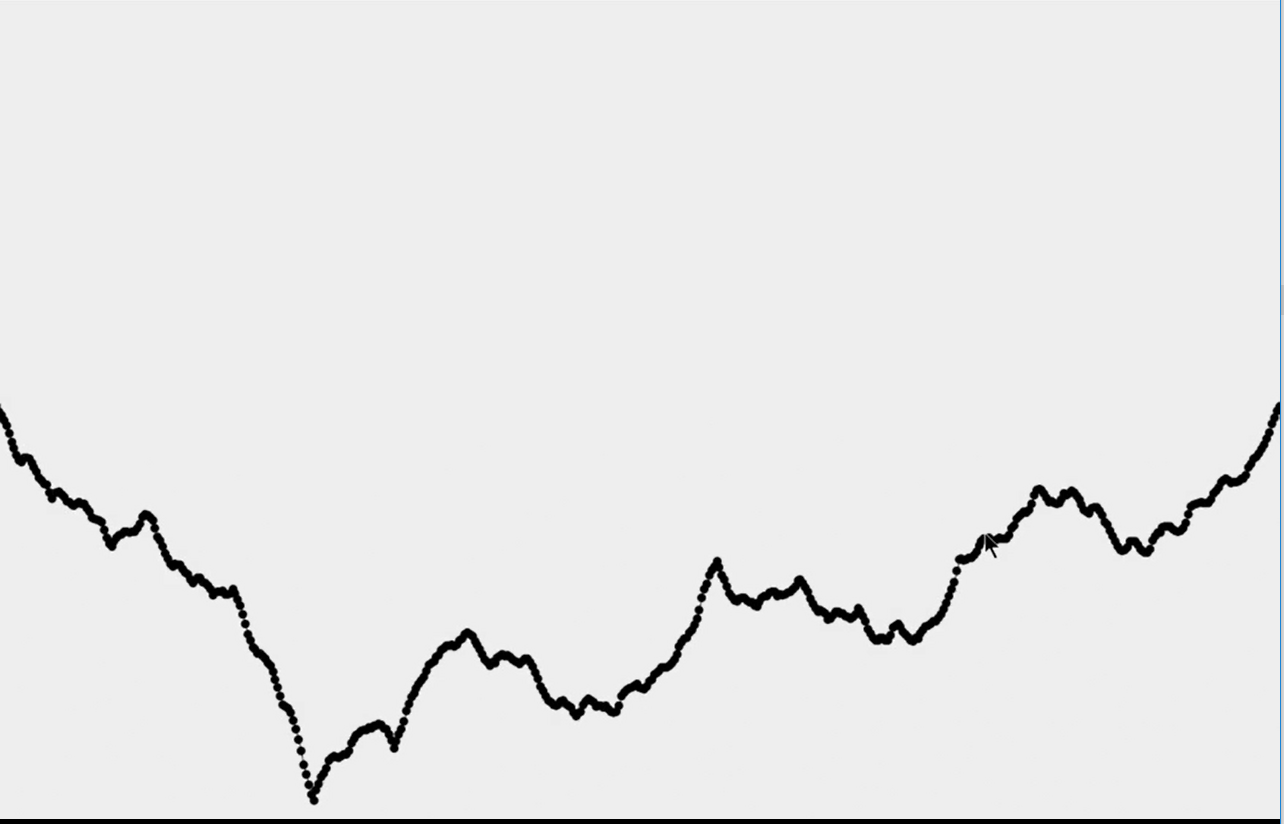
\includegraphics[scale = 0.5]{Capture.png}\\
.gif also included in submission, named ani.gif

\section{Question 3: Grids and Recursion}
\subsection{Non-Recursive Method}
\begin{lstlisting}
C:\Users\bp001\Documents\EECS223\HW5>java Grid
Enter a direction for a step (s=straight, l=left, r=right, q=quit):
s
Enter a direction for a step (s=straight, l=left, r=right, q=quit):
l
Enter a direction for a step (s=straight, l=left, r=right, q=quit):
r
Enter a direction for a step (s=straight, l=left, r=right, q=quit):
l
Enter a direction for a step (s=straight, l=left, r=right, q=quit):
l
Enter a direction for a step (s=straight, l=left, r=right, q=quit):
s
Enter a direction for a step (s=straight, l=left, r=right, q=quit):
q
Turn 180 degrees
Take a step and remain straight
Take a step and turn right
Take a step and turn right
Take a step and turn left
Take a step and turn right
Take a step and remain straight
You have arrived where you started!
\end{lstlisting}
\subsection{Recursive Method}
\begin{lstlisting}
C:\Users\bp001\Documents\EECS223\HW5>java RecursiveGrid
Enter a direction for a step (s=straight, l=left, r=right, q=quit):
s
Enter a direction for a step (s=straight, l=left, r=right, q=quit):
l
Enter a direction for a step (s=straight, l=left, r=right, q=quit):
r
Enter a direction for a step (s=straight, l=left, r=right, q=quit):
l
Enter a direction for a step (s=straight, l=left, r=right, q=quit):
l
Enter a direction for a step (s=straight, l=left, r=right, q=quit):
s
Enter a direction for a step (s=straight, l=left, r=right, q=quit):
q
Turn 180 degrees
Take a step and remain straight
Take a step and turn right
Take a step and turn right
Take a step and turn left
Take a step and turn right
Take a step and remain straight
You have arrived where you started!
\end{lstlisting}

\end{document}